\documentclass[12pt]{article}

\usepackage{cite}
\usepackage{listings}
\usepackage{multicol}
\usepackage{newtxtext}
\usepackage{setspace}
\usepackage{sectsty}
\usepackage{booktabs}
\usepackage{graphicx}
\usepackage{amsmath}
\usepackage{amssymb}
\usepackage{algorithm}
\usepackage{algpseudocode}
\usepackage{xcolor}
\usepackage[T1]{fontenc}
\usepackage[numbib]{tocbibind}
\usepackage[lmargin=1.25in,rmargin=1.25in,tmargin=1.0in,bmargin=1.0in]{geometry}

\definecolor{codegreen}{rgb}{0,0.6,0}
\definecolor{codegray}{rgb}{0.5,0.5,0.5}
\definecolor{codepurple}{rgb}{0.58,0,0.82}
\definecolor{backcolour}{rgb}{0.95,0.95,0.92}

\lstdefinestyle{thesiscodelisting}{
    keywordstyle=\color{magenta},
    numberstyle=\tiny\color{codegray},
    stringstyle=\color{green},
    basicstyle=\ttfamily\footnotesize,
    breakatwhitespace=false,
    breaklines=true,
    captionpos=b,
    keepspaces=true,
    showspaces=false,
    showstringspaces=false,
    showtabs=false,
}

\lstset{style=thesiscodelisting}

% \settowidth{\parindent}{}

\begin{document}
% Riddle thesis title page
\begin{center}
    \LARGE
    \textbf{
        \textit{
            Language Modeling of Aviation Communications\\
        }
    }

    \vspace*{0.2in}

    \normalsize
    by\\
    \textit{Aaron Van De Brook}\\

    \vspace*{0.25in}

\end{center}
This thesis was prepared under the direction of the candidate's thesis
committee chairman, \underline{Dr.~Jianhua Liu}, Department of \underline{Electrical Engineering \&
    Computer Science}, and has been approved by the members of the thesis committee.
It was submitted to the Department of Electrical Engineering \& Computer Science
and was accepted in partial fulfillment of the requirements for the degree of
Masters of Electrical \& Computer Engineering.

% Signature lines/committee members
\begin{center}
    \begin{minipage}{3in}
        \vspace*{0.25in}
        THESIS COMMITTEE:\\
        \vspace*{0.25in}
        \hrule
        \vspace*{2pt}
        Jianhua Liu, Ph.D.\\
        Committee Chairman\\
        \vspace*{0.75in}
        \hrule
        \vspace*{2pt}
        Prashant Shekhar, Ph.D.\\
        Committee Member\\
        \vspace*{0.75in}
        \hrule
        \vspace*{2pt}
        Andrew Schneider\\
        Committee Member\\
        \vspace*{0.75in}
        \hrule
        \vspace*{2pt}
        Massood Towhidnejad, Ph.D.\\
        Department Chair, Electrical Engineering \& Computer Science\\
        \vspace*{0.75in}
        \hrule
        \vspace*{2pt}
        Associate Vice President for Academics
    \end{minipage}
\end{center}
\newpage
\tableofcontents
\newpage
\doublespacing{}

\section{Notation and Terminology}
% TODO: proper writing, bulleted list for now
This section is included for the sake of clarity throughout this thesis. In pursuit of that, there are a few terms and notations that are defined
below.

Set notation is used in parts of this thesis, particularly in equations and algorithms, to convey mathematical concepts. With that being said, the
shorthand below is defined
\begin{equation*}
    A; x := A \cup \{x\}
\end{equation*}

\noindent
as adding the element $x$, of its own set, to the set $A$.

The following words (in bold) are used throughout the thesis as they relate to language modeling and are defined concretely as follows:
\begin{itemize}
    \item A \textbf{sequence} shall be defined as a set of tokens (distinct from a sentence)
    \item A \textbf{token} shall be defined as the smallest, fundamental component of a sequence (distinct from characters and words)
    \item The rules for the formation of tokens from a sentence (and into sequences) shall be defined by tokenization algorithms (section
          \ref{sec:tokenizers})
    \item The definition of \textbf{words} and \textbf{sentences} follow from that of the English language
    \item The \textbf{vocabulary}, \textbf{inventory}, \textbf{index}, and \textbf{word list} of a model shall be semantically identical
\end{itemize}
\newpage

\section{Abstract}\label{sec:abstract}


\section{Introduction}\label{sec:introduction}
There have been noticeable and significant advancements in the general domain of artificial intelligence (AI) recently. Natural language processing
and language modeling technologies, in particular, have made tremendous advances over the past two decades achieving performance levels good enough to
be brought to consumer facing products such as personal assistants, search engines, phones, televisions, etc. Due to the success in the general
domain, applications have begun to spin-off into problem-specific domains, such as (and most notably for this work) aviation. For example, several
speech recognition systems with rule- and machine learning-based natural language processing, inference, and semantic extraction algorithms have been
implemented at EUROCONTROL simulation centers in Europe to train air traffic controllers and study the potential effects of AI augmented air traffic
management (ATM) systems on controller workloads. Preliminary studies have found that AI augmented ATM systems not only reduce controller workloads
but also reduce fuel consumption of aircraft by optimizing aircraft routes in the airspace and reducing departure/arrival times thereby reducing fuel
consumption~\cite{helmke_quantifying_2017}.

At the time of this writing, the current focus of general machine learning and deep learning algorithms in the language modeling domains has been on a
variety of deep learning methods/architectures, namely; recurrent, convolutional, and transformer neural networks due to the availability of large
natural language corpora corpora such as WikiText~\cite{merity_pointer_2016} and IMDB~\cite{maas_learning_2011}. In contrast to the general domain,
the aviation domain still prefers, and sees much success with, traditional machine learning models for language modeling applications. Typically, the
most prevalent of the traditional models are Hidden Markov models, Gaussian Mixture models, and/or in conjunction with word lattices, N-grams, and/or
rule-based approaches depending on the application and operating environment of the models. The most likely reason for this divergence between the
domains is the difference and relative lack of labeled data in the aviation domain. By comparison, the largest corpora in the general domain is either
WikiText or the BookCorpus which contain trillions of tokens whereas, for aviation, the largest corpus is Air Traffic Control Complete with
approximately 26 hours of labeled data amounting to just over 300,000 tokens\footnote{Air Traffic Control Complete has approximately 70 hours of
    audio data, however, about 26 hours of the 70 are labeled.}. This disparity in data availability is exacerbated by the fact that aviation English
uses a specialized vocabulary in addition to specialized pronunciation for some words to enhance understandability in a radiotelephonic (R/T)
medium~\cite{paltridge_handbook_2013}, making it significantly more difficult to transcribe/label data as it requires transcribers to have domain
knowledge and experience in order to create effective transcriptions. The medium of communication along with the environment in which the
communication occurs i.e.~a noisy and possibly low fidelity medium\footnote{Depending on the equipment used to transmit and receive R/T
    communications.} combined with a noisy and active communication environment---an active flight deck (influenced by wind, engine noise, etc.~) or
an active Air Traffic Control (ATC) tower (other people/controllers conversing or communicating in the background)---and a rapid rate of speech
\cite{paltridge_handbook_2013}, further contributing to the difficulty in understanding and therefore transcribing aviation English.


% connect complexity of aviation english to utility/necessity of NLP models (ASR and LM) in the aviation domain
The potential for speech recognition and language modeling algorithms to reach better than human performance (for example, the SQuAD benchmark has
recorded results consistently better than human since 2019\footnote{https://rajpurkar.github.io/SQuAD-explorer/})~\cite{zhang_ai_2022} suggests that
these NLP algorithms could have high utility in the aviation domain. If they can achieve better-than-human performance in the aviation domain, and be
used in conjunction with pilot and air traffic controller systems, they could easily boost efficiency, reduce workloads, and reduce and/or mitigate
errors during normal operations.

The methods and results laid out in this work were done with the intention of creating a streamlined process for training and testing deep learning
based NLP methods, specifically automatic speech recognition and text-based language models. The results from the language models suggest that the
volume of text used to train the language models is not yet sufficient to produce results akin to those in the conversational and/or literary English
domains. However, the automatic speech recognition models were able to achieve near state-of-the-art results and, according to the literature review,
better than other deep learning-based approaches in the aviation domain.

\section{Literature Review}\label{sec:lit_review}
% from thesis proposal; revise and add to this as more references are used
% transformer history (background)
The transformer neural network architecture was proposed in 2017 for Neural Machine Translation tasks and immediately achieved
state-of-the-art (28.4 BLEU on WMT 2014 English-to-German; 41.8 BLEU on WMT English-to-French datasets)\cite{vaswani_attention_2017}. Transformer
architectures have been found to be extremely effective at learning representations and understandings of languages to predict token probabilities as
opposed to transforming one language into another\cite{devlin_bert_2019,liu_roberta_2019}. Transformers have also been found to be very effective at
other NLP-related tasks such as prompt completion and sentiment analysis among others (i.e.~auto-regressive and sequence classification tasks,
respectively)\cite{lewis_bart_2019,radford_improving_2018}. Devlin et al.~proposed pretraining methods such as masked language
modeling and next sentence prediction to improve natural language understanding for downstream tasks \cite{devlin_bert_2019}, which was further
expanded upon by Liu et al.~by training longer, with larger batch sizes, and removing the next sentence prediction task \cite{liu_roberta_2019}.

% tokenizer algorithms
In language modeling and natural language processing tasks more generally, the out-of-vocabulary (OOV) problem is prevalent and has been addressed by
the introduction of tokenizer algorithms. WordPiece and Byte Pair Encoding have been used to solve OOV problems while simultaneously minimizing
vocabulary sizes and maximizing the likelihood of tokens in sequences \cite{wu_googles_2016,schuster_japanese_2012,sennrich_neural_2016}.

% LMs and NLP in aero. domain
Various natural language processing methods have been applied to the aviation domain to help deal with miscommunications
and try to mitigate safety incidents\cite{ragnarsdottir_language_2003,tanguy_natural_2016,madeira_machine_2021}.
Some machine learning approaches have been implemented to analyze the text in aviation incident and safety reports to predict
contributing factors and topic models\cite{tanguy_natural_2016,madeira_machine_2021}. An ASR system with NLP post-processing
has also been proposed to analyze Air-Traffic communications and condense significant features (e.g.~weather, runway, and
heading info) into an XML language structure\cite{ragnarsdottir_language_2003}. Transformer language models such as BERT and RoBERTa have been applied
to notice to airmen (NOTAM) messages to perform named entity recognition (NER) tasks, translation tasks (between notations; e.g.~NOTAM notation to
Airlang to make parsing tasks easier) and reduce the workload for pilots during long-haul flights\cite{arnold_knowledge_2022}. Transformer models
have also been used for speaker role identification tasks in the aviation domain (e.g.~identifying pilot versus controller in communications),
specifically, a pretrained BERT model was used and fine-tuned on problem specific data and compared to other models that performed well at speaker
and role identification tasks in general\cite{guo_comparative_2022}.

% ASR context (suggest some need for semi-supervised approaches and therefore LMs)
Automatic speech recognition is seeing increased use in aviation for tasks such as transcription, callsign detection, speaker identification,
etc. A majority of these approaches use machine learning approaches (as opposed to deep learning) where acoustic, pronunciation, and language
modeling is used to transcribe speech
\cite{guo_comparative_2022,smidl_air_2019,zuluaga-gomez_automatic_2020,badrinath_automatic_2022,hofbauer_atcosim_2008,helmke_quantifying_2017}.
Language models have been used in the general domain (both neural and machine learning-based approaches) to boost the performance of speech
recognition models \cite{han_contextnet_2020,kriman_quartznet_2020,majumdar_citrinet_2021}. Machine learning-based language models, usually N-grams
and word lattices have also been used in the aviation domain alongside semi-supervised approaches to automatic speech recognition to leverage
unlabeled data, however, none of the developed methodologies use neural language models for their applications
\cite{zuluaga-gomez_contextual_2021,srinivasamurthy_semi-supervised_2017,badrinath_automatic_2022}.

% differences in language (transcripts vs literary english), narrow model selection
The use of the English language in aviation has been shown to be sufficiently different enough to be classified under its own category (aviation
English) \cite{paltridge_handbook_2013}. The issue with using pretrained checkpoints of transformer-based language models is characterizing the
similarity (or, conversely, the difference) between literary English and aviation English. If the two domains are sufficiently different, then
training the pretrained models on aviation English data would amount to transfer learning between specific domains. Transfer learning between text
domains has been shown to be possible even with data volumes significantly lower than the original data used to train the models
\cite{raffel_exploring_2020}. Although, Yadlowsky et al.~recently showed that if problem domains are sufficiently different, model pretraining on data
considered out-of-domain will have negative effects on model performance \cite{yadlowsky_pretraining_2023}.


\section{Data Sources}\label{sec:data_source}
There are four corpora used in this work. The datasets are primarily speech corpora intended either for automatic speech recognition research in the
domain of aviation communications, linguistics research in aviation English, or both. All data in all four corpora include both recordings and
transcriptions, audio and text, respectively. The transcriptions are used to pretrain and train the language models and tokenizers (described in
sections \ref{sec:language_modeling} and \ref{sec:tokenizers}).

The four corpora that were selected and used for this work are briefly described below. Further analysis is performed in section \ref{sec:data_analysis}.

\subsection{Air Traffic Control Complete}\label{sec:atcc}
The Air Traffic Control Complete (ATCC) corpus is a speech corpus consisting of audio recordings with corresponding transcriptions.
ATCC is a collection of three smaller corpora recorded at Dallas-Fort Worth, Logan International, and Washington National airports and
transcribed by current or former air traffic controllers familiar with the respective areas. Audio data was recorded through the placement of VHF
antennae configured to monitor several frequencies at each airport, such as arrival, departure, approach, ground, etc. The types of frequencies
monitored vary by airport, but the presence of departure, approach, and ground frequencies is relatively consistent across subcorpora~\cite{godfrey_air_1994}.
% TODO: data length/size

\subsection{ATCO2}\label{sec:atco2}
The ATCO2 dataset is a speech corpus that consists of audio communications at Prague and Brno airports, in Czechia, along with corresponding
transcriptions. The speech recordings and transcripts are crowd sourced from volunteers. The dataset was created and labeled, in part, as an English
language detection corpus, however, the labeling also includes transcripts of speech segments which makes it practical for ASR and language model
development in addition to language detection (although in this work it is only used for ASR and LM development)~\cite{szoke_detecting_2021}.
% TODO: data length/size


\subsection{Air Traffic Control Simulation}\label{sec:atcosim}
The Air Traffic Control Simulation (ATCOSIM) corpus is a speech corpus consisting of audio recordings and corresponding transcriptions.
The data was recorded at a air traffic control simulation center in Bretigny-sur-Orge, France, specifically the EUROCONTROL Experimental Centre.
In this data, only the controllers' voices are included and therefore the transcripts only include the controller's side of each interaction.
The audio data was transcribed by one person, trained according to the guidelines and formatting requirements of the corpus. After all data was
transcribed, it was reviewed and corrected and any remaining problems were reviewed by an operational air traffic controller and
resolved\cite{hofbauer_atcosim_2008}.
% TODO: data length/size

\subsection{ZCU CZ ATC Corpus}\label{sec:zcu_atc}
The ZCU CZ ATC corpus consists of audio recordings and corresponding transcripts in the Czech airspace. Both controller and pilot sides of the
communications are included in this data. Annotations were created by experienced transcribers/annotators and labeled samples were randomly selected
for review during the annotation process. After the dataset was completely labeled, all samples were checked, corrected, and
unified\cite{smidl_air_2019}.
% TODO: data length/size

\section{Data Processing}\label{sec:data_processing}
All of the corpora listed above (see~\ref{sec:data_source}) are created at different times, for different purposes, and by different authors.
As a result, the data in these corpora all have different formats and need to be processed into a common format to be used together, with the goal
being to essentially create a ``super-corpus'' that includes all the corpora listed above (i.e., a superset of the other corpora).

All data was processed in Python using primarily built-in functions/modules\footnote{The \lstinline|re| and \lstinline|xml| modules were also used
    although these are built into most Python distributions by default.}. The text data is extracted from the corpus transcripts by parsing from the
corpora-specific formats where necessary i.e.~Lisp in ATCC, XML in ATCO2 and ZCU CZ ATC, and plain text in ATCOSIM, the transcriber annotations
are removed where necessary\footnote{A copy of the original data is made, then the annotations are removed from the copy.}, and the resulting text
is written to a file in the standard corpus format (an ASCII text file with one line in the file corresponding to one sample from the corpus) to a
file.

\subsection{Handling Spelling Errors \& Inconsistencies}\label{sec:spelling_errors}
By the nature of the data labeling process, there are bound to be spelling errors introduced by the annotators during corpora creation. This gets
exacerbated by the aggregation of several corpora with varying controls for correcting spelling errors and inconsistencies. Nearly all of the errors
are recoverable/correctable given context. For example, ``possibility of \textbf{tornado's}'' should clearly have been ``possibility of
\textbf{tornadoes}'', changing the possessive form of ``tornado'' to the plural form. There are also instances of spelling conventions that are
consistent within corpora, but become inconsistent when the corpora are combined.

% 22 spelling errors
Manually reviewing every sample in the corpus is unrealistic considering that there are over 50,000 data samples and would be subject the same
human error that introduced those errors in the first place. Instead, the frequency of occurrence of tokens in the corpora combined with manual review
thereafter, was used to detect and correct the most common errors. Tokens with the lowest frequency across corpora were manually reviewed and
corrected where necessary. An \(A \rightarrow B\) mapping system was used to correct the errors, where \(A\) is the erroneous token and \(B\) is the
corrected or replaced token. A total of 22 unique errors were detected and subsequently corrected or removed using this method, although multiple
instances of those errors typically occurred.

% hesitations, cut off words, different kinds of filled pauses
The mapping system described above is also used to modify within corpora conventions to be consistent across corpora. Three areas are addressed here:
hesitations, cut-off or partial words, and filled pauses within speech. These areas are defined differently between the four corpora, which makes
unifying the transcripts difficult. Hesitations, for example, are defined by one corpus as any incomplete or non-english speech sounds and left
completely undefined by another (despite annotators making notes about hesitations). The way in which hesitations, pauses, and partial words are
transcribed differs between corpora as well. Two corpora prescribe special tokens to these phenomena such as ``[hes]'', ``[hesitation]'', ``<pause>'',
or similar, while the others transcribe the data as it sounds (i.e., ``uh'', ``eh'', or ``er'' for filled pauses and ``cir-'' or ``cir+'' for
instances that were cut-off mid pronunciation). In order to facilitate the unification of the transcripts for all four corpora, the conventions for
transcribing these phenomena are redefined below:

\begin{table}[h!]
    \centering
    \begin{tabular}{l p{0.65\linewidth}}
        \toprule
        Phenomenon               & Definition                                                                                                              \\
        \midrule
        Hesitations              & Instances of hesitation for which the specific realization is not defined (usually some special token is used instead). \\
        \midrule
        Partial \& cut-off words & Partially pronounced words are indicated by a hyphen character where the pronunciation of the word is missing.          \\
        \midrule
        Filled pauses            & Hesitations with a verbal component that has been described or otherwise defined by the corpus/annotator.               \\
        \bottomrule
    \end{tabular}
    \caption{Speech/transcription phenomena with corresponding convention for transcribing or translating, depending on the corpus being processed.}
    \label{tab:phenomena_definitions}
\end{table}



\begin{table}[h!]
    \centering
    \begin{tabular}{l l}
        \toprule
        Phenomenon                   & Convention for representation \\
        \midrule
        Hesitations                  & [HES]                         \\
        \midrule
        Partial \& cut-off words     & -                             \\
        \midrule
        Filled pauses (open-mouth)   & uh, um, ah                    \\
        \midrule
        Filled pauses (closed-mouth) & hm, mhm                       \\
        \bottomrule
    \end{tabular}
    \caption{Conventions for transcript representation/translation of phenomena to keep transcripts consistent across corpora.}
    \label{tab:phenomena_conventions}
\end{table}

A special token is used to represent hesitations when no other context regarding the realization of hesitation is present. If other corpora use a
special token to represent hesitations, it is translated to match the convention in table~\ref{tab:phenomena_conventions}. Partial/cut-off words
are represented with a hyphen (-) at the point where the pronounced word is cut off. For example, if the last syllable of ``approaching'' is cut
mid transmission, it would be represented in the transcript as ``approa-'' or, likewise, if the first syllable is cut off, it would be written as
``-roaching''. Lastly, if there is enough information in the original transcript to indicate the realization of a hesitation, it is represented by
the most appropriate token from ``Filled pauses'' in table~\ref{tab:phenomena_conventions}.

One of the intended downstream use cases of the language models developed from this work is decoding speech recognition predictions into transcripts,
so including as much data as possible regarding the realization of spoken words is useful given the context. The \lstinline|[HES]| token is used as a
catch-all, fallback token in the case that no knowledge can be extracted about the utterance from the transcript.

\section{Data Analysis}\label{sec:data_analysis}
% sequence lengths, unique tokens, total number of tokens, total number of samples, breakdown by each dataset
Relevant corpora statistics were observed or calculated and are presented in Table~\ref{tab:corpora_stats}. This includes the number of samples in
the corpus, mean sequence length per sample in the corpus, the number of unique tokens in the corpus, and the total number of tokens in the corpus.
The same statistics were also calculated across corpora, since all four corpora will be combined for training and testing the language and speech
recognition models. Note that this is based on the raw data after loading and unifying the corpora, prior to preprocessing for model training/testing
and outlier removal.


\begin{table}[h!]
    \centering
    \begin{tabular}{l r r r r}
        \toprule
        \textbf{Corpus} & \textbf{Samples} & \textbf{Mean Sequence Length (\(\pm \sigma\))} & \textbf{Unique Tokens} & \textbf{Tokens} \\
        \midrule
        ATCC            & 29,862           & \(11.90 \pm 7.22\)                             & 2,209                  & 355,473         \\
        ATCO2           & 874              & \(12.28 \pm 4.12\)                             & 786                    & 10,733          \\
        ATCOSIM         & 9,544            & \(11.23 \pm 4.12\)                             & 823                    & 107,153         \\
        ZCU CZ ATC      & 14,435           & \(10.05 \pm 5.50\)                             & 2,983                  & 145,107         \\
        \midrule
        Total           & 54,715           & \(11.30 \pm 6.36\)                             & 5,040                  & 618,466         \\
        \bottomrule
    \end{tabular}
    \caption{The number of samples, mean sequence length, number of unique tokens, and total number of tokens by corpus, including the cumulative
        total across all corpora.}
    \label{tab:corpora_stats}
\end{table}

The ATCC and ZCU CZ ATC corpora make up a significant portion of the data, ATCC alone makes up more than half (approximately 54\%) of the combined
data, and ATCC and ZCU CZ ATC together make up approximately 81\% of the data. The sequence lengths of the samples are fairly consistent across
corpora with at most about an 18\% percent difference between sequence lengths. The number of unique tokens does not scale additively to the
combined corpora, which is as expected. Considering that aviation English generally conforms to and follows ICAO phraseology standards we would expect
that many terms would be shared across corpora with the exception of geographic/location specific terms, such as city, landmark, airport, and airline
names, etc.~that typically vary across regions.

\subsection{Outlier Detection and Analysis}\label{sec:outliers}
The Local Outlier Factor (LOF) algorithm~\cite{breunig_lof_2000} was used to detect and remove outliers in the corpora for further analysis. The
sequence lengths of the data samples were used to determine outliers. Since all four corpora are aggregated, LOF analysis was performed on the
aggregated data instead of on the individual corpora.

Sci-Kit Learn's implementation of the LOF
algorithm was used with a value of \(N = 35\) for \(N\) neighbors in the K-Nearest Neighbors algorithm and Minkowski distance for distance
metrics/calculations (in this case, since \(p=2\), Euclidean distance is effectively used for distance calculations). A total of 47 samples were
detected as outliers and removed for analysis and are summarized in table~\ref{tab:outlier_stats}.

\begin{table}[h!]
    \centering
    \begin{tabular}{l | r}
        \toprule
        \multicolumn{2}{c}{Outlier Properties}   \\
        \midrule
        \textbf{Mean Sequence Length}    & 47.30 \\
        \textbf{Std of Sequence Length}  & 11.82 \\
        \textbf{Minimum Sequence Length} & 38    \\
        \textbf{Maximum Sequence Length} & 73    \\
        \textbf{\# Samples}              & 47    \\
        \bottomrule
    \end{tabular}
    \caption{Mean, standard deviation, minimum, and maximum sequence length of samples detected as outliers.}
    \label{tab:outlier_stats}
\end{table}

Although all of the outliers have higher sequence lengths than the typical sequence lengths of the other samples in the data, going the through
the outlying samples manually and reviewing each reveals that, for the most part, the samples are typical albeit somewhat complex communications.
With the exception of four outliers, all of the samples labeled as outlying by the LOF algorithm were kept in the data.

\section{Language Modeling}\label{sec:language_modeling}
% bert, roberta
% n-gram
This section introduces the chosen language model architectures as well as their pretrained checkpoints, if one is used. Two transformer-based
architectures are used, BERT and RoBERTa, and statistical/machine learning-based approaches such as N-gram and word lattices.

The transformers are pre-trained using the same masked language modeling (MLM) objective presented in Devlin et al.~\cite{devlin_bert_2019} to train
BERT for bidirectional encoding representation and likewise in Liu et al.~\cite{liu_roberta_2019} for training RoBERTa. Given the results of the
RoBERTa pretraining and downstream task training thereafter, it was initially decided to eliminate the next sentence prediction (NSP) task as it was
used in BERT, however, their results suggest that the success of the MLM-only approach was due to the increase in batch and overall data
size~\cite{liu_roberta_2019}. Taking this into account, along with the very limited amount of data available in the domain of aviation an NSP
pretraining task was implemented where possible\footnote{Only about half of the data (only the data from ATCC, since it is continuous recordings of
    the airspace) is in a format that enables us to extract the turn taking phenomenon that is present in most air-traffic communications.} to improve
its pretraining results. MLM and NSP pretraining are explained more in-depth in section \ref{sec:bert}, below.

\subsection{N-Gram}\label{sec:ngram}
An N-gram language model estimates the probability of a token occurring in a sequence based on the \(N\) tokens preceding or succeeding that token.
In other words, for a sequence, $X$, of $T$ tokens

\begin{equation}\label{eq:ngram_sequence}
    X = \mbox{$w_1$, $w_2$, $w_3$, ..., $w_T$}
\end{equation}

\noindent
the probability of a token, $w_i$, occurring in the sequence can be represented as

\begin{equation}\label{eq:ngram_preceding}
    \begin{gathered}
        P(w_i) = P(w_i|w_{i-1},w_{i-2},w_{i-3},...,w_{i-N}) \\
        P(w_i) = \prod_{j=i-1}^{i-N} P(w_j)
    \end{gathered}
\end{equation}

\noindent
or for the case of succeeding tokens (looking ahead $N$ tokens)

\begin{equation}\label{eq:ngram_succeeding}
    \begin{gathered}
        P(w_i) = P(w_i|w_{i+1},w_{i+2},w_{i+3},...,w_{i+N}) \\
        P(w_i) = \prod_{j=i+1}^{i+N} P(w_j)
    \end{gathered}
\end{equation}

\noindent
where $N$ is the number of preceding (or succeeding) tokens. Since the $N$ preceding tokens\footnote{The most common use case for an N-gram model is
    the preceding tokens.} are needed prior to the estimation of the probability of $w_i$, N-grams are sometimes referred to as left-associative
models (in a left-to-right language).

The probability of a token occurring anywhere in a sequence (referred to as $w_j$ in equations \ref{eq:ngram_preceding} and \ref{eq:ngram_succeeding})
is determined statistically as the number occurrences of a token in a corpus divided by the total number of tokens in the corpus.

\begin{equation}\label{eq:ngram_prob_wj}
    P(w) = \frac{\textit{occurrences}(w)}{D_{tokens}}
\end{equation}

\noindent
where $P(w)$ is the probability of a token, $w$, occurring anywhere in the corpus, $\textit{occurrences}(w)$ is the number of times of a specific
token appears in the corpus, and $D_{tokens}$ is total number of tokens in the corpus, $D$. Computationally, the process of determining the
probabilities of the individual tokens in the corpus is typically referred to as training or fitting the N-gram model.

$N$ is a predetermined value based on model or application requirements and while it can technically take any value from one to infinity, its
usability becomes very limited at the minimum sequence length in the corpus and unusable at any value at or above the maximum sequence length.
Depending on implementation, the time and resources required to train a model with a large value of $N$ can be very expensive. The most common values
for $N$ in the literature are one, two, and three, sometimes called unigrams, bigrams, and trigrams, respectively.

\subsection{BERT}\label{sec:bert}
The purpose of BERT (Bidirectional Encoder Representations from Transformers) is to represent tokens in text sequences in relation to the tokens
preceding and following the token in question. Whereas an N-gram model represents token probabilities based on the $N$ tokens preceding a specific
token or, conversely, the $N$ tokens succeeding said token, BERT models are able to predict the probability of a token based on both preceding and
succeeding tokens, thus the bidirectionality novelty.

\textbf{Masked Language Modeling}. The ability of BERT to represent text in a bidirectional context is achieved through the Masked Language Modeling
(MLM) pretraining task~\cite{devlin_bert_2019}. MLM pretraining choses a certain percentage of token positions at random for prediction, then tokens
are replaced with either a ``mask'' token, a random token, or the original token according to preconfigured probabilities (BERT used 80\% for the mask
token, 10\% for random tokens, and 10\% for the original/unchanged token). The original token is then predicted with cross-entropy loss.

\textbf{Next Sentence Prediction}. NSP is meant to support downstream tasks, while MLM conditions the model to represent tokens within sentences, NSP
is meant to condition the model to understand relationships between sentences/sequences. Since BERTs training set consists primarily of literary works
and excerpts from Wikipedia, the model simply predicts whether two sentences appear together (one after the other) in the original text. Instead of a
single input sequence, the input consists of two sequences separated by a ``separation'' token and beginning with a ``classification'' token, these
are represented by \lstinline|[SEP]| and \lstinline|[CLS]|, respectively in Devlin et al.~\cite{devlin_bert_2019}.

For symmetry between pretraining tasks, the special tokens specifying the beginning and end of input sequences are shared between tasks. For both MLM
and NSP objectives, input sequences always start with a classification token and end with a separation token (see figure \ref{fig:bert_mlm_input_example}).

\begin{figure}[h!]
    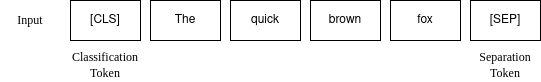
\includegraphics[width=\linewidth]{figures/BERT_MLM_input.png}
    \caption{An example of an input sequence for a masked language modeling pretraining task. Modified from Devlin et al.~\cite{devlin_bert_2019}.}
    \label{fig:bert_mlm_input_example}
\end{figure}

\noindent
Likewise, NSP inputs always begin with a classification token and each input sequence is concatenated with a separation token terminating each
sequence (see figure \ref{fig:bert_nsp_input_example}).

\begin{figure}[h!]
    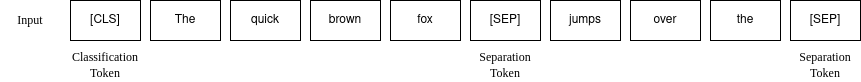
\includegraphics[width=\linewidth]{figures/BERT_NSP_input.png}
    \caption{An example of an input sequence for a next sentence prediction pretraining task.}
    \label{fig:bert_nsp_input_example}
\end{figure}

\subsection{RoBERTa}\label{sec:roberta}
As the name implies, RoBERTa, is an iteration on BERT (described in section \ref{sec:bert}, above). The results from Liu et
al.~\cite{liu_roberta_2019} indicate that BERT was initially significantly undertrained, so by training longer, with larger batch sizes, on
longer sequences, and dynamically changing the masking pattern applied to the MLM pretraining task, the performance of BERT was improved. The new
checkpoint of this version of BERT was therefore called RoBERTa (Robustly Optimized BERT Pretraining Approach).

The pretraining methodology introduced by RoBERTa eliminated the NSP pretraining task that was originally used in BERT and opted instead to increase
the quantity of training data along with the batch sizes in addition to training the model longer. Lastly, there is a small difference in the
construction of input sequences as compared to BERT; input sequences always begin with a classification token (\lstinline|[CLS]|) and individual
segments are separated by a separation token (\lstinline|[SEP]|). Rather than having sequences end with a separation token as well, they are
terminated with an end of sequence token (\lstinline|[EOS]|). See equation \ref{eq:roberta_input_example} modified from Liu et
al.~\cite{liu_roberta_2019}, below.

\begin{equation}\label{eq:roberta_input_example}
    \mbox{[CLS], $x_1$, $x_2$, ..., $x_N$, [SEP], $y_1$, $y_2$, ..., $y_M$, [EOS]}
\end{equation}

% \section{Speech Recognition}\label{sec:speech_recognition}
% Automatic speech recognition (ASR) or simply speech recognition is the process of translating spoken language to text i.e.~transcribing spoken
% language. There have been a myriad of approaches to ASR problems, including, but not limited to rule-based, machine learning, and deep learning
% methods. For the purposes of this work, we will focus primarily on deep learning approaches to ASR tasks with a specific focus on transcribing
% spoken language in aviation (following from the data accumulated, processed, and analyzed in sections \ref{sec:data_source},
% \ref{sec:data_processing}, and \ref{sec:data_analysis}).

% Three ASR architectures were chosen due to their success in the conversational English domain and ease of reproducing results. Nvidia maintains a
% Python package called Neural Modules (shortened to NeMo) with PyTorch implementations of many well-performing ASR models\footnote{Performance of these
%     models can be seen in their respective papers (referenced hereafter).}, including the three models used in this work and described in more detail
% below \cite{kuchaiev_nemo_2019}.

% Although the internal processing of data varies between architectures, the format of the models input and output is generally the same. ASR models
% have seen much success and performance gains through the use of Mel-frequency Cepstral Coefficients (MFCCs), so the audio files provided by the
% corpora used in this work were processed and resampled into the same format, then the MFCCs are extracted according to the process
% in~\cite{sahidullah_design_2012}. The MFCCs are then used as input to the ASR models. Each model outputs a probability distribution of characters or
% tokens (depending on the vocabulary the ASR model is initialized with) over a segment of audio. All the ASR models used are trained with a
% Connectionist Temporal Classification (CTC) loss function~\cite{graves_connectionist_2006}.

% \subsection{Jasper}\label{sec:jasper}
% Jasper is a family of end-to-end convolutional neural networks (CNNs) developed by NVIDIA to replace traditional ASR models that use separately
% learned components for each stage of the pipeline (acoustic, pronunciation, language modeling, etc.) \cite{li_jasper_2019}.

% Jasper models are designed with $B$ blocks and $R$ sub-blocks and are named accordingly as \textit{Jasper $B\mbox{x}R$} models. The Jasper
% architecture also contains four extra convolutional blocks, one for preprocessing and three for postprocessing (see figure \ref{fig:jasper}). Each
% convolutional sub-block contains one dimensional convolutions. Li et al.~trained and tested a Jasper 10x5 model that produced state-of-the-art
% results on the LibriSpeech, Wall Street Journal, and Fisher+Switchboard speech corpora \cite{li_jasper_2019}.

% \begin{figure}[h!]
%     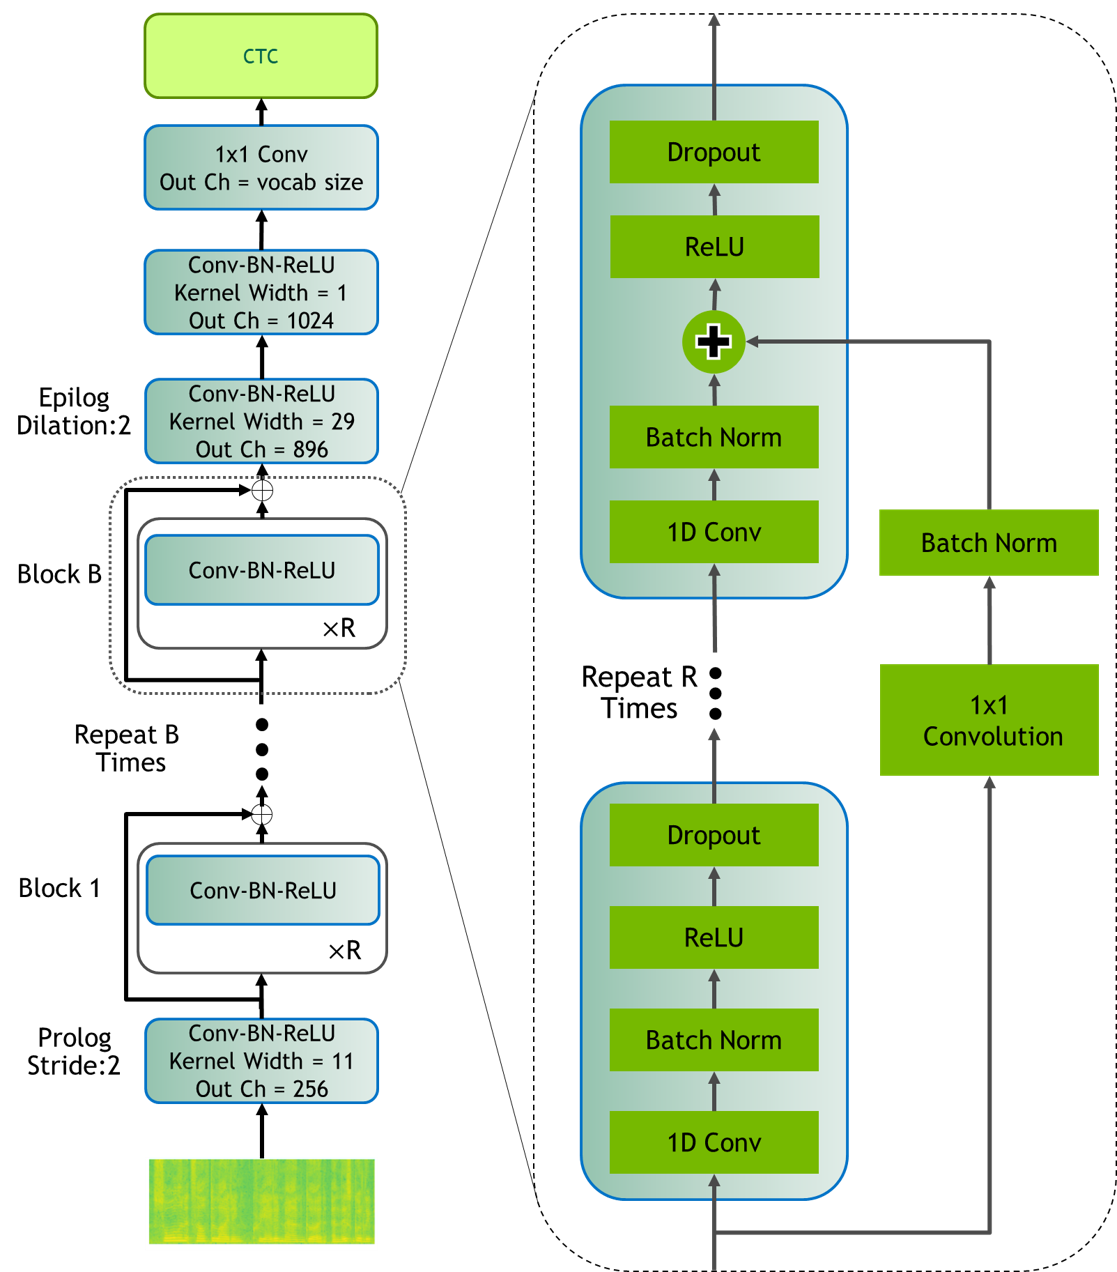
\includegraphics[width=\linewidth]{figures/jasper_vertical.png}
%     \caption{Block diagram of the Jasper architecture. Copied from Li et al.~\cite{li_jasper_2019}.}
%     \label{fig:jasper}
% \end{figure}

% \subsection{QuartzNet}\label{sec:quartznet}
% The QuartzNet architecture is based on Jasper with some key modifications, namely, that the one dimensional convolutions are replaced with ``one
% dimensional time-channel separable convolutions''. As with Jasper, QuartzNet models are denoted as \textit{QuartzNet $B\mbox{x}R$}, however, blocks
% are repeated $S$ times and have a certain number of input and output channels, $c_{in}$ and $c_{out}$, respectively.

% In Kriman et al.~experiments with QuartzNet were conducted on the LibriSpeech and Wall Street Journal speech corpora and achieved near state-of-the-art
% performance on both. A transfer learning experiment was also performed (transferring between corpora). The model was initially trained on LibriSpeech
% and Mozilla Common Voice, then fine-tuned on the Wall Street Journal corpus and also achieved near state-of-the-art results \cite{kriman_quartznet_2020}.
% These results suggest that the QuartzNet architecture not only performs well on in-domain tasks, but can generalize and fine-tune well on related
% data.

% \begin{figure}[h!]
%     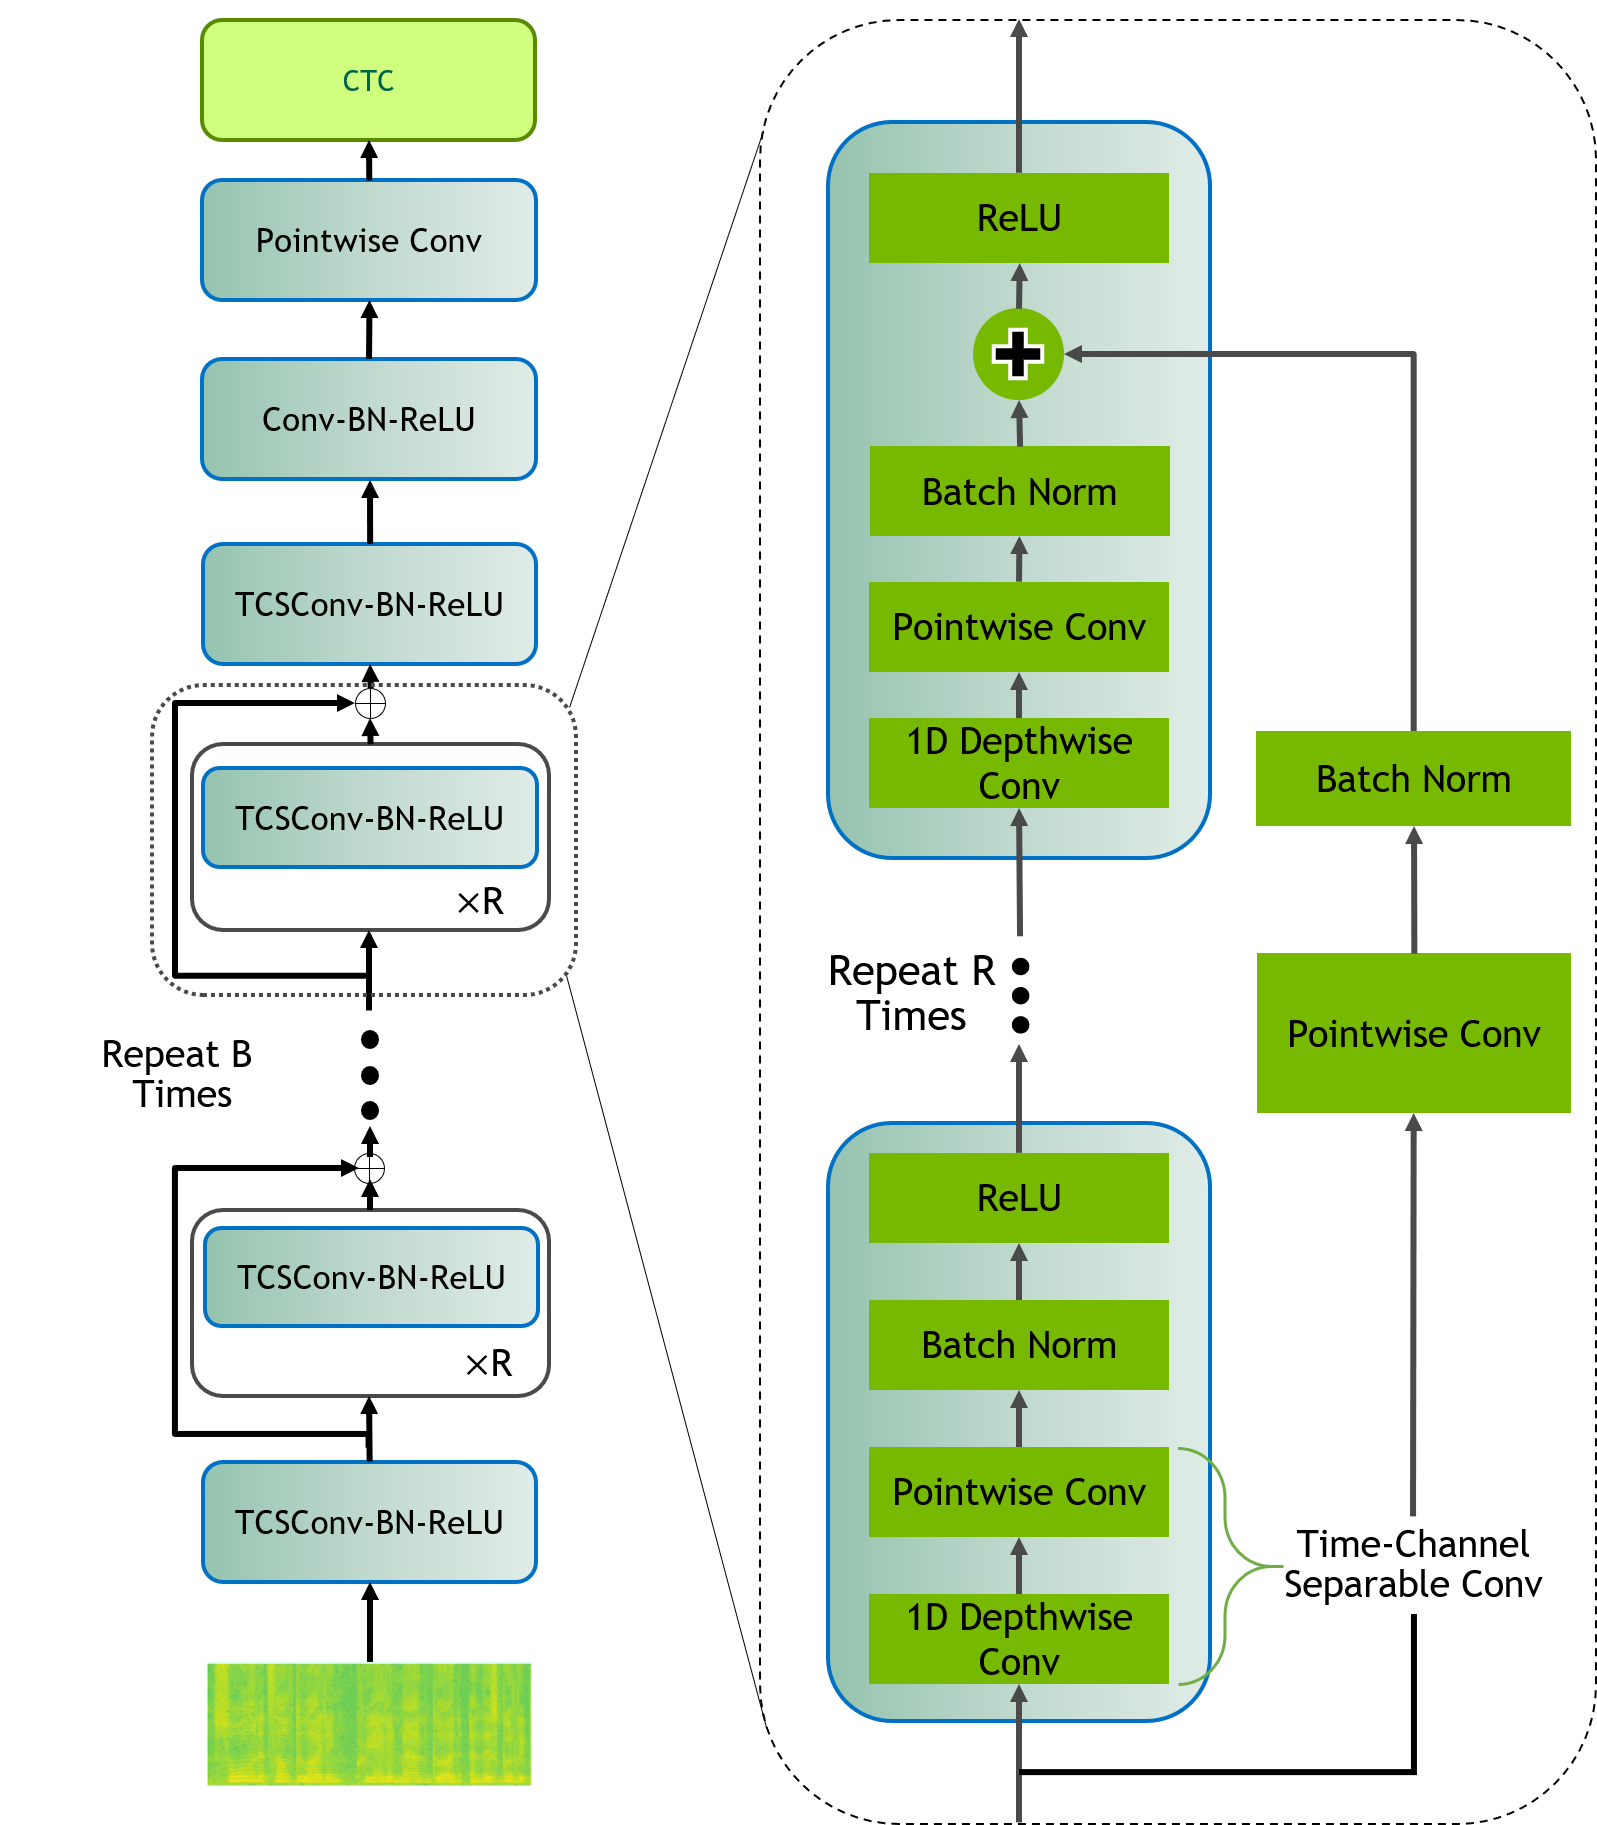
\includegraphics[width=\linewidth]{figures/quartz_vertical.png}
%     \caption{Block diagram of the QuartzNet architecture. Copied from Kriman et al.~\cite{kriman_quartznet_2020}.}
%     \label{fig:quartznet}
% \end{figure}

% \subsection{Citrinet}\label{sec:citrinet}
% Citrinet is an end-to-end CNN based on QuartzNet (and thus Jasper) and augmented with one dimensional Squeeze and Excitation modules
% \cite{hu_squeeze-and-excitation_2018}. Citrinet models are denoted as \textit{Citrinet $B$x$R$x$C$} with $B$ representing the number of blocks, $R$
% representing the number of repeated sub-blocks, and $C$ representing the number of channels. Similarly to Jasper and QuartzNet, Citrinet has a set of
% prolog and epilog blocks, in this case one of each, the first and last-most blocks, respectively. The core of the model architecture consists of three
% ``mega blocks'', which are themselves made up of seven QuartzNet blocks that are repeated $R$ times along with a Squeeze and Excitation module at the
% end of the block. The value of $C$ follows from that of QuartzNet (section \ref{sec:quartznet}, above; $c_{in}\mbox{x}c_{out}$) \cite{majumdar_citrinet_2021}.

% \begin{figure}[h!]
%     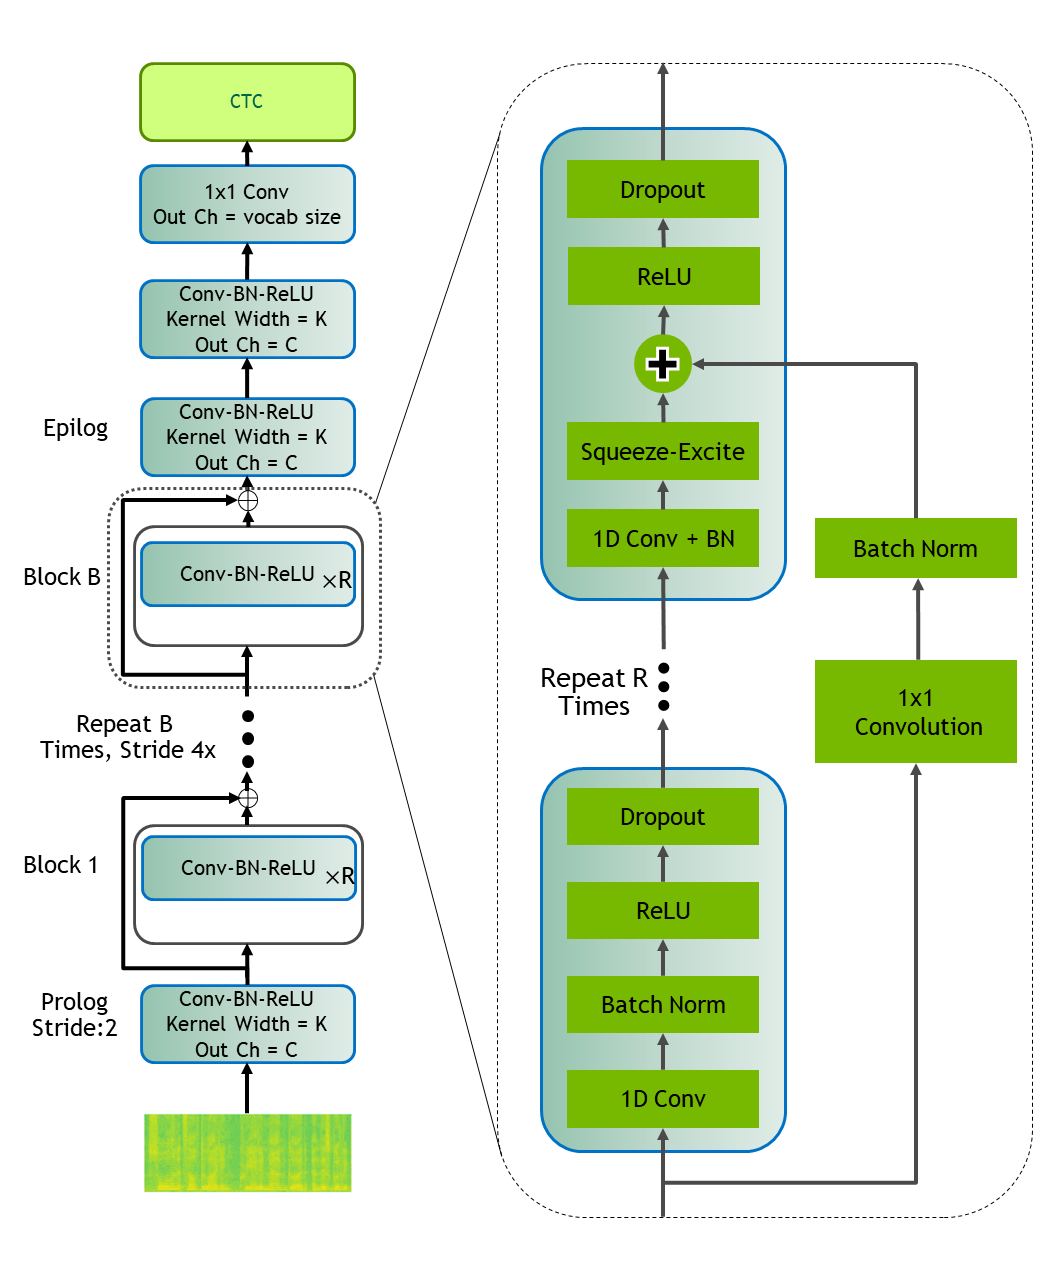
\includegraphics[width=\linewidth]{figures/citrinet_vertical.png}
%     \caption{Block diagram of the Citrinet architecture. Copied from Majumdar et al.~\cite{majumdar_citrinet_2021}.}
% \end{figure}

% Citrinet also uses a WordPiece tokenizer (described in more detail in section \ref{sec:wordpiece}), typically with a vocabulary size of 1024 tokens
% (or word pieces) in the experiments performed by Majumdar et al. The results from the experiments showed model performance on ASR transcription tasks
% near or better than the other state-of-the-art models that the \textit{Citrinet-1024} was compared against \cite{majumdar_citrinet_2021}.

\section{Tokenization Algorithms}\label{sec:tokenizers}
% present and explain the tokenization algorithms used (possibly which models they correspond to)
Tokenization is the process of separating or segmenting words in sentences into their component ``tokens''. The tokenized version of a sentence is
referred to as a sequence. The rules by which the tokens are created or segmented depend entirely on the algorithm used. The simplest and most
intuitive way to do this by creating tokens based on whitespace i.e., each ``word'' in the corpus is  treated as a token\footnote{The Huggingface
    Tokenizer library implements this as the \lstinline|WordLevel| tokenizer.}. While this is simple and works in theory, it does not take into
account the fact that not every word in a language will occur in a corpus. The inevitable possibility for a tokenizer to see a word that was not in
the original training corpus is known as the out-of-vocabulary (OOV) problem~\cite{wu_googles_2016}. The OOV problem has been addressed by several
different algorithms. For brevity's sake, only the tokenization algorithms used by the models in this work are defined and explained.

\subsection{WordLevel}\label{sec:wordlevel}
The WordLevel tokenization algorithm, mentioned briefly as an introductory example above, is the most technically simple algorithm among those
introduced in this section. Tokens are extrapolated from words in a sentence based on the whitespace separating each word. This means that
contractions, hyphenations, etc.~are treated as their own words i.e.~ ``you'', ``you're'', and ``you've'' are all seen as unique, distinct words that
are tokenized and mapped to their own integral representations.

In order to map individual tokens to numerical values or IDs, an index of the words that appear in a corpus must be created. The numerical values for
each token are derived from this index. For the WordLevel algorithm, this process is referred to as the training the tokenizer model.

The first step of the training procedure is to index any specified special tokens, such as mask, classification, or separation tokens (this is why
special tokens often have low-valued token IDs). The second step is to split the sentences in the training data into individual words. This is done
by splitting each string based on whitespace, in other words the tokenizer treats sentences as lists of words delimited by space characters. Lastly,
the tokenizer iterates through each word in each sentence, indexing new words as it finds them, until all sentences in the training corpus have been
analyzed. Token IDs are then derived based on the position of the word in the tokenizer index or vocabulary.

\begin{algorithm}
    \caption{Training procedure for the WordLevel tokenizer.}
    \label{alg:wordlevel_training}
    \begin{algorithmic}
        \State $D = \{s_1, s_2, ..., s_N\}$
        \Comment{$D$, $s_i$, and $N$ are corpus, sentence, and corpus length}
        \State $V \gets \{\varnothing\}$
        \Comment{$V$ is the tokenizer vocabulary and is initialized to the empty set}\\

        \For{$s \in D$}
        \State Split $s$ into words using whitespace as a delimiter such that
        \State $W=\{w_1, w_2, ... w_M\}$
        \Comment{$w$ and $M$ are words and sentence length}\\

        \For{$w \in W$}
        \If{$w \notin V$}
        \State $V \gets V;w$
        \Comment{Add $w$ to the vocabulary}
        \EndIf
        \EndFor
        \EndFor
    \end{algorithmic}
\end{algorithm}

Table \ref{tab:wordlevel_tokenization_example} shows the different representations of the input sentence over the course of the tokenization process.

\begin{table}[h!]
    \centering
    \begin{tabular}{l l}
        \toprule
        Tokenization stage & Representation                                                                            \\
        \midrule
        Input string:      & ``the quick brown fox jumps over the lazy dog''                                           \\
        Tokenized string:  & [``the'', ``quick'', ``brown'', ``fox'', ``jumps'', ``over'', ``the'', ``lazy'', ``dog''] \\
        Integral mapping:  & [5, 16, 9, 12, 13, 15, 5, 14, 11]                                                         \\
        \bottomrule
    \end{tabular}
    \caption{A simple example of the tokenization process of the WordLevel tokenization algorithm.}
    \label{tab:wordlevel_tokenization_example}
\end{table}

\noindent
The simplicity of the algorithm speaks for itself and serves as a good introduction to tokenization as well as an illustrative example of the OOV
problem. Note that the values of the integers representing the tokens are determined based on the order in which the tokens are seen during the
training process (special tokens are defined and therefore seen first), so these results are completely reproducible as long as the data appears in
the same order.

The tokenization of words with shared roots but different suffixes is shown in table \ref{tab:wordlevel_tokenization_shared_roots_example}.

\begin{table}[h!]
    \centering
    \begin{tabular}{l l}
        \toprule
        Tokenization stage & Representation                    \\
        \midrule
        Input string:      & ``you you're you've''             \\
        Tokenized string:  & [``you'', ``you're'', ``you've''] \\
        Integral mapping:  & [18, 19, 20]                      \\
        \bottomrule
    \end{tabular}
    \caption{The results of tokenizing three words with the same roots and differing suffixes.}
    \label{tab:wordlevel_tokenization_shared_roots_example}
\end{table}

\noindent
Clearly all three words are seen as independent and unique words by the tokenizer, since they are mapped to their own integer representations.

The tokenizer used to generate the examples in tables \ref{tab:wordlevel_tokenization_example} and
\ref{tab:wordlevel_tokenization_shared_roots_example} was trained on two sentences, notably lacking the word ``you'll''. Running the tokenizer on the
word ``you'll'' alone results in the following output:

\begin{table}[h!]
    \centering
    \begin{tabular}{l l}
        \toprule
        Tokenization stage & Representation \\
        \midrule
        Input string:      & ``you'll''     \\
        Tokenized string:  & [``[UNK]'']    \\
        Integral mapping:  & [0]            \\
        \bottomrule
    \end{tabular}
    \caption{Results of running the WordLevel tokenizer on an unknown word similar to some of those in the training data.}
    \label{tab:wordlevel_unk_word}
\end{table}

\noindent
Although the word shares a root with some of the words in the training data (``you'', ``you're'', and ``you've'') and is semantically very similar,
the tokenizer does not recognize the word at all (represented by the ``[UNK]'' or unknown token). This word would be considered out-of-vocabulary
since it did not appear in the training data and thus reveals one of the major downsides of this algorithm, as mentioned in section
\ref{sec:tokenizers}. This problem can be alleviated to some extent by modifying the preprocessing strategy of the tokenizer to partition contracted
words into their component parts e.g.~the word ``you're'' would be partitioned to \lstinline|[``you'', ``''', ``re'']|, however, it eventually
reappears, for example, when using the past, present, and future tenses of a verb (e.g.~``go'' and ``goes'' in the training data, then encountering
the future tense: ``going'').

\subsection{WordPiece}\label{sec:wordpiece}
% Wu et al. 2016; Schuster and Nakajima 2012
The WordPiece algorithm was developed by Schuster and Nakajima in 2012~\cite{schuster_japanese_2012} as a word segmentation algorithm for language
modeling in Japanese and Korean voice search systems. It is further used by Wu et al.~\cite{wu_googles_2016} for neural machine translation tasks. The
algorithm demonstrated proficiency and increased performance for the models used in both tasks and effectively addressed the OOV problem.

One of the primary stipulations for this algorithm is effective and efficient handling of OOV words such that none are produced during normal
operation. To achieve this, during training, the vocabulary of the tokenizer is initialized to a basic set of characters; since WordPiece is designed
to be language agnostic, the initial vocabulary is specified as all basic unicode characters (for the chosen language) in addition to all ASCII
characters.

The training procedure works by iterating over the vocabulary, combining two word units to maximize the likelihood over the training data, and
repeating until one of two stop conditions are reached:

\begin{enumerate}
    \item The predefined word limit is reached
    \item The increase in likelihood falls below the predefined threshold
\end{enumerate}

\noindent
The training procedure is simple, but computationally expensive. Schuster and Nakajima calculated the time complexity of the algorithm at $O(K^2)$
where $K$ is the current size of the vocabulary~\cite{schuster_japanese_2012}. Due to the high time complexity of the algorithm, the authors suggest
the following considerations to reduce the computational complexity:

\begin{itemize}
    \item Test only pairs that actually exist in the training data
    \item Test only pairs with a significant chance of being best (high prior likelihood)
    \item Combine several clustering steps into a single iteration (for groups of pairs which don't affect each other)
    \item Only modify language model counts for the affected entries
\end{itemize}

Table \ref{tab:wordpiece_tokenization_example}, below, shows an example of a WordPiece tokenizer model output on a sentence that was seen during the
training procedure (trained on the same data as the WordLevel tokenizer in section \ref{sec:wordlevel}).

\begin{table}[h!]
    \centering
    \begin{tabular}{l l}
        \toprule
        Tokenization stage & Representation                                                                            \\
        \midrule
        Input string:      & ``the quick brown fox jumps over the lazy dog''                                           \\
        Tokenized string:  & [``the'', ``quick'', ``brown'', ``fox'', ``jumps'', ``over'', ``the'', ``lazy'', ``dog''] \\
        Integral mapping:  & [59, 98, 95, 88, 97, 91, 59, 90, 87]                                                      \\
        \bottomrule
    \end{tabular}
    \caption{A simple example of the tokenization process of the WordPiece algorithm.}
    \label{tab:wordpiece_tokenization_example}
\end{table}

\noindent
Since this sentence was in the training data, the segmentation is identical to that of the WordLevel tokenizer in table
\ref{tab:wordlevel_tokenization_example}, however, tokenization of similar words e.g.~words with shared roots or similar contractions are handled
differently as in table \ref{tab:wordpiece_tokenization_shared_roots_example}.

\begin{table}[h!]
    \centering
    \begin{tabular}{l l}
        \toprule
        Tokenization stage & Representation                                            \\
        \midrule
        Input string:      & ``you you're you've''                                     \\
        Tokenized string:  & [``you'', ``you'', ``''', ``re'', ``you'', ``''', ``ve''] \\
        Integral mapping:  & [56, 56, 5, 71, 56, 5, 72]                                \\
        \bottomrule
    \end{tabular}
    \caption{Example of WordPiece tokenization of words with shared roots and differing suffixes.}
    \label{tab:wordpiece_tokenization_shared_roots_example}
\end{table}

\noindent
Since each word has a shared root word in the contractions (as well as an apostrophe separating the contraction), the tokenizer segments each word and
represents them as groups of small, more common (thus with higher probabilities of occurring) tokens. Additionally, the WordPiece algorithm
effectively handles OOV words. Take the OOV in table \ref{tab:wordpiece_unk_word_similar} with a shared root and similar contraction as those in table
\ref{tab:wordpiece_tokenization_shared_roots_example}, which appear in the training data.

\begin{table}[h!]
    \centering
    \begin{tabular}{l l}
        \toprule
        Tokenization stage & Representation                     \\
        \midrule
        Input string:      & ``you'll''                         \\
        Tokenized string:  & [``you'', ``''', ``l'', ``\#\#l''] \\
        Integral mapping:  & [56, 5, 17, 54]                    \\
        \bottomrule
    \end{tabular}
    \caption{WordPiece tokenization of an unknown word similar to some of those in the training data.}
    \label{tab:wordpiece_unk_word_similar}
\end{table}

\noindent
Since the base of the contraction, ``you'', occurs in the training data as well as the apostrophe in the contraction, so the tokenizer segments those
parts of the word as tokens. The last part of the word, ``ll'', does not appear at all in the training data, so it is broken down into its component
characters which are represented as ``l'' (beginning of a word) and ``\#\#l'' (segmented part of a word that should be concatenated to the previous
token when they are recombined). Comparing this to the results of the WordLevel tokenizer output on the same word in table
\ref{tab:wordlevel_unk_word}, the WordPiece algorithm sidesteps the OOV problem for words similar to those in the trining corpus and, according to
the output of the WordPiece tokenizer in table \ref{tab:wordpiece_unk_word}, for words unlike those in the training corpus.

\begin{table}[h!]
    \centering
    \begin{tabular}{l l}
        \toprule
        Tokenization stage & Representation                                                             \\
        \midrule
        Input string:      & ``anything''                                                               \\
        Tokenized string:  & [``an'', ``\#\#y'', ``\#\#t'', ``\#\#h'', ``\#\#i'', ``\#\#n'', ``\#\#g''] \\
        Integral mapping:  & [61, 49, 37, 53, 32, 36, 39]                                               \\
        \bottomrule
    \end{tabular}
    \caption{WordPiece tokenization of a word that does not appear in the training data and is not similar to any of the words in the tokenizer
        vocabulary.}
    \label{tab:wordpiece_unk_word}
\end{table}

\subsection{Byte-Pair Encoding}\label{sec:bpe}
% Sennrich et al. 2016; Gage 1994
The Byte-Pair Encoding (BPE) tokenizer algorithm was adapted from a data compression algorithm by Gage 1994~\cite{gage_feb94_1994}. The data compression
algorithm works by replacing common pairs of bytes in data with an unused byte to reduce the overall size of the data. The tokenization algorithm
works under the same principle, merging frequent pairs of characters or tokens into one token~\cite{sennrich_neural_2016}.

The vocabulary of the tokenizer is initialized to the base set of characters (letters, numbers, punctuation, etc.~). The training procedure begins by
counting all pairs (``A'', ``B'') of characters that appear in the training data and combines the most frequently occurring pair into one token
(``A'', ``B'' $\rightarrow$ ``AB''). This process repeats until a specified vocabulary size has been reached (or a specified number of merge
operations have occurred; the final vocabulary size is equal to the base character set plus the number of merge operations). Algorithm
\ref{alg:bep_training} shows a minimal Python implementation for the BPE training procedure.

\begin{algorithm}[h!]
    \caption{BPE training algorithm implementation in Python. Modified from Sennrich et al.~\cite{sennrich_neural_2016}.}
    \label{alg:bep_training}
    \begin{lstlisting}[language=Python]
import re, collections

def get_stats(vocab):
    pairs = collections.defaultdict(int)
    for word, freq in vocab.items():
        symbols = word.split()
        for i in range(len(symbols)-1):
            pairs[symbols[i], symbols[i+1]] += freq
        return pairs
def merge_vocab(pair, v_in):
    v_out = {}
    bigram = re.escape(' '.join(pair))
    p = re.compile(r'(?<!\S)' + bigram + r'(?!\S)')
    for word in v_in:
        w_out = p.sub(''.join(pair), word)
        v_out[w_out] = v_in[word]
    return v_out

vocab = {...}
num_merges = 10
for i in range(num_merges):
    pairs = get_stats(vocab)
    best = max(pairs, key=pairs.get)
    vocab = merge_vocab(best, vocab)
    print(best)
    \end{lstlisting}
\end{algorithm}

Finally, comparing the tokenization process to the WordLevel and WordPiece algorithms, we can see that the outputs of the algorithm are nearly
identical when the sentences being tokenized have words that appear in the training data (i.e.~the BPE outputs in tables
\ref{tab:bpe_tokenization_example} and \ref{tab:bpe_shared_roots_example} are almost identical to the WordPiece output in tables
\ref{tab:wordpiece_tokenization_example} and \ref{tab:wordpiece_tokenization_shared_roots_example} with the exception of the numerical representation
of the tokens) and very similar to that of the WordLevel tokenizer.

\begin{table}[h!]
    \centering
    \begin{tabular}{l l}
        \toprule
        Tokenization stage & Representation                                                                            \\
        \midrule
        Input string:      & ``the quick brown fox jumps over the lazy dog''                                           \\
        Tokenized string:  & [``the'', ``quick'', ``brown'', ``fox'', ``jumps'', ``over'', ``the'', ``lazy'', ``dog''] \\
        Integral mapping:  & [36, 70, 72, 66, 74, 69, 36, 68, 64]                                                      \\
        \bottomrule
    \end{tabular}
    \caption{The Byte-Pair Encoding tokenizer output for a string that appears in the training data.}
    \label{tab:bpe_tokenization_example}
\end{table}

\begin{table}[h!]
    \centering
    \begin{tabular}{l l}
        \toprule
        Tokenization stage & Representation                                            \\
        \midrule
        Input string:      & ``you you're you've''                                     \\
        Tokenized string:  & [``you'', ``you'', ``''', ``re'', ``you'', ``''', ``ve''] \\
        Integral mapping:  & [34, 34, 5, 33, 34, 5, 37]                                \\
        \bottomrule
    \end{tabular}
    \caption{Byte-Pair Encoding tokenizer output for semantically similar words with shared roots.}
    \label{tab:bpe_shared_roots_example}
\end{table}

\noindent
Now, testing the BPE algorithm on words that did not appear in the training data, it is clear that the BPE algorithm effectively deals with and
processes OOV words (tables \ref{tab:bpe_unk_similar} and \ref{tab:bpe_unk}), even when no subunits of the word appear in the training data (table
\ref{tab:bpe_unk}).

\begin{table}[h!]
    \centering
    \begin{tabular}{l l}
        \toprule
        Tokenization stage & Representation                 \\
        \midrule
        Input string:      & ``you'll''                     \\
        Tokenized string:  & [``you'', ``''', ``l'', ``l''] \\
        Integral mapping:  & [34, 5, 17, 17]                \\
        \bottomrule
    \end{tabular}
    \caption{Byte-Pair Encoding tokenizer output for a word that did not appear in the training data, but is similar to some of the words in the
        training data.}
    \label{tab:bpe_unk_similar}
\end{table}

\begin{table}[h!]
    \centering
    \begin{tabular}{l l}
        \toprule
        Tokenization stage & Representation                                     \\
        \midrule
        Input string:      & ``anything''                                       \\
        Tokenized string:  & [``an'', ``y'', ``t'', ``h'', ``i'', ``n'', ``g''] \\
        Integral mapping:  & [39, 30, 25, 13, 14, 19, 12]                       \\
        \bottomrule
    \end{tabular}
    \caption{Byte-Pair Encoding tokenizer output for a word that did not appear in the training data and is not similar to any words in the training
        data.}
    \label{tab:bpe_unk}
\end{table}

\textbf{Byte-Level Byte-Pair Encoding}. This is a subset of the BPE algorithm that is also commonly used for NLP tasks such as neural machine
translation, language modeling, and generative tasks (GPT-2 uses a byte-level BPE tokenizer~\cite{radford_language_2019}). As Huggingface's
\lstinline|tokenizers| library implements it, this is a preprocessing step for the tokenizer model that maps all bytes in a string/sentence to their
own unique and visible character. Functionally, byte-level BPE is nearly identical to standard BPE models with the main exception being that the
beginning of word symbol is actually rendered and represented by a visible character in the tokenized sequence (see table
\ref{tab:byte_level_bpe_example}).

\begin{table}[h!]
    \centering
    \begin{tabular}{l l}
        \toprule
        Tokenization stage & Representation                                            \\
        \midrule
        Input string:      & ``anything''                                              \\
        Tokenized string:  & [``Ġa'', ``n'', ``y'', ``t'', ``h'', ``i'', ``n'', ``g''] \\
        Integral mapping:  & [36, 19, 30, 25, 13, 14, 19, 12]                          \\
        \bottomrule
    \end{tabular}
    \caption{Example of the output of a byte-level Byte-Pair Encoding tokenizer with the begging of a word represented with the ``Ġ'' character.}
    \label{tab:byte_level_bpe_example}
\end{table}

\section{Discussion}\label{sec:discussion}
Considering the success of deep learning models with transformer-based architectures for language modeling and natural language processing (NLP)
tasks, more generally, in the conversational and literary English domains, it follows that transformer architectures should see widespread use in the
domain of aviation English for domain-specific NLP tasks, however, according to the literature, transformer-based language models have seen sparse
use. The most notable example of the use of a transformer deep neural network is the application of BERT for knowledge extraction from notice to
airmen (NOTAM) messages \cite{arnold_knowledge_2022}.

\subsection{Language Model Pretraining}\label{sec:lm_pretraining}
A standard masked language modeling training procedure is used to pretrain the language models, as described in section \ref{sec:bert}. Tokens are
masked at random with at a uniform probability of 0.2. Input sequences are padded to the maximum length allowed by the model and truncated to the
maximum length, if greater. The maximum sequence length for BERT and RoBERTa models is 512 tokens \cite{devlin_bert_2019,liu_roberta_2019}. Based on
the data analysis in section \ref{sec:data_analysis}, there are few, if any, samples that meet or exceed the maximum sequence length for BERT and
RoBERTa models.

The models are trained with the \textit{AdamW} optimizer \cite{loshchilov_decoupled_2019} using the hyperparameters in table \ref{tab:optim_params}
based on the most effective pretraining configuration presented in \cite{devlin_bert_2019} and \cite{liu_roberta_2019}.

\begin{table}[h!]
    \centering
    \begin{tabular}{l r}
        \toprule
        Hyperparameter & Value              \\
        \midrule
        $\beta_1$      & $0.9$              \\
        $\beta_2$      & $0.98$             \\
        $\epsilon$     & $1 \times 10^{-6}$ \\
        Learning Rate  & $4 \times 10^{-5}$ \\
        Weight Decay   & $0.01$             \\
        \bottomrule
    \end{tabular}
    \caption{\textit{AdamW} hyperparameters for training BERT and RoBERTa models.}
    \label{tab:optim_params}
\end{table}

A train/test split of 70\% and 30\% and a validation split of 10\% of the training data was used for each model. The blank models (the models that are
trained from randomly initialized weights; also referred to as being trained from scratch) were trained for 200 epochs and the pretrained models were
trained for 100 epochs. These values were chosen through trial and error, monitoring the perplexity and loss curves of the
validation set to ensure that the pretraining does not result in net negative effects on the loss and perplexity of the model (i.e.~to ensure that the
models are not overfitting to the training data). Batch sizes of 16 were used for training all four models; this was the maximum batch size that
worked reliably with the hardware available to train the models\footnote{Values larger than 16 would sometimes cause CUDA Out of Memory errors, so 16
    was used to ensure all models trained continuously without error and/or interruption.}.

\begin{table}
    \centering
    \begin{tabular}{l r r}
        \toprule
        Corpus split & Split size (\%) & Samples \\
        \midrule
        Train        & 68.99           & 34,470  \\
        Validation   & 6.999           & 3,830   \\
        Test         & 30.01           & 16,415  \\
        \bottomrule
    \end{tabular}
    \caption{Number of samples and percentage of overall corpus by split.}
    \label{tab:corpus_splits}
\end{table}

\subsection{Performance Metrics}\label{sec:performance_metrics}
As mentioned previously, perplexity and cross-entropy loss (often shortened to loss) are used to track the performance of the model on the training
and validation sets, per epoch, while training. Cross-entropy loss is defined by the following equation:

\begin{equation}\label{eq:cross_entropy_loss}
    \begin{gathered}
        \mathcal{L}(x, y) = \{\mbox{$l_1$, $l_2$, ..., $l_N$}\}^T\\
        l_n = -\log \left[\frac{\exp(x_{n,y_n})}{\sum_{c=1}^{C}\exp(x_{n,c})}\right]
    \end{gathered}
\end{equation}

\noindent
Where $x$ and $y$ are $N \times 1$ vectors representing the inputs and labels, respectively, for each sample in the batch. $N$ is the number of
samples in the batch, $l_n$ is the loss for an individual sample, $n$, in the batch, and $C$ is the number of class labels. For the purpose of
language modeling, the set of class labels is equivalent to the vocabulary of the tokenizer (and thus the language model). Numerical labels will
correspond to token IDs.

Perplexity is related to the probability of a token appearing in a sequence. It is used as a measure of how well a language model can predict tokens
in a sequence and is defined by the equation below:

\begin{equation}\label{eq:perplexity}
    \begin{gathered}
        X = \{x_1, x_2, ..., x_N\}\\
        \mbox{PPL} = \exp\left[\frac{\sum_{i=1}^N - \log_2 x_i}{N}\right]
    \end{gathered}
\end{equation}

\noindent
Where $X$ is an input sequence, $N$ is the length of the sequence, and $x_i$ is an individual token in the sequence, $X$.

\subsection{Pretraining Results}\label{sec:pretraining_results}
With the metrics above defined, an analysis of the results of the model pretraining can be performed. The objective of the pretraining procedure is to
build the models' understanding of the structure of the text, in this case transcripts of air-traffic communications. By tracking the average
cross-entropy loss (loss) and perplexity (PPL) during training, we can estimate how well (and how correctly) the models are predicting tokens and if
the models are effectively ``understanding'' token placements in sequences.

Graphs of the training loss (average loss over the samples/batches in the training partition of the corpus) are presented in figure
\ref{fig:training_loss}.

\begin{figure}[h!]
    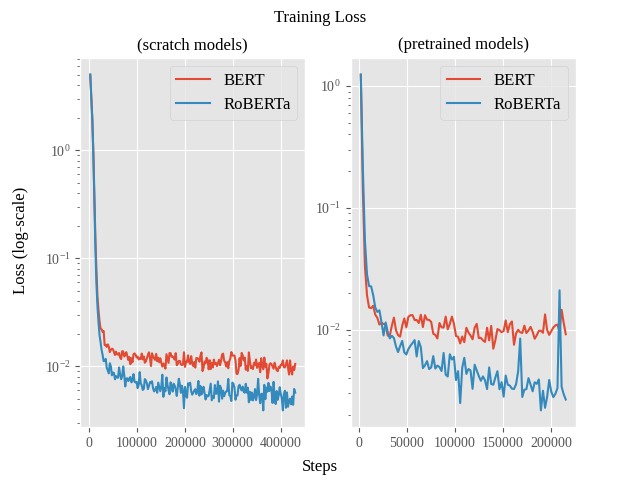
\includegraphics[width=\linewidth]{figures/training_loss.png}
    \caption{Loss on the training partition of the corpus over time (steps).}
    \label{fig:training_loss}
\end{figure}

\noindent
Both classes of models (scratch and pretrained) quickly reach a steady state in terms of loss although the initial loss values are significantly
different. It is notable that the pretrained models start with a significantly lower loss, about 1.3, compared to models trained from scratch, which
started with a loss value of just over 5.0. This initially indicates that the models are training well and beginning to converge on either local or
global minima.

The perplexity of the models on the training data yields interesting results (figure \ref{fig:training_ppl}). Although the pretrained models have a
more stable curve over time, the models trained from scratch result in a significantly lower perplexity. Note the difference in the scales on the
y-axis in figure \ref{fig:training_ppl}; the final perplexity value of each language model trained from scratch is at least two orders of magnitude
lower than that of the pretrained models.

\begin{figure}[h!]
    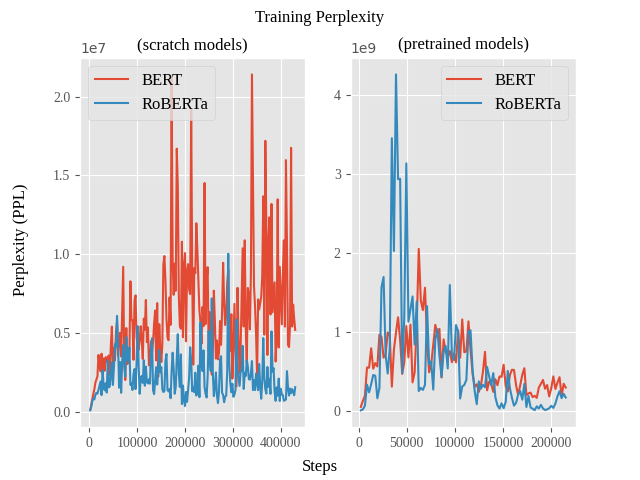
\includegraphics[width=\linewidth]{figures/training_ppl.png}
    \caption{Language model perplexity on the training partition of the corpus over time (steps). Note the scales on the y axes.}
    \label{fig:training_ppl}
\end{figure}

\noindent
At the end of training, the BERT and RoBERTa models trained from scratch had perplexity values of $0.52\times 10^7$ and $0.16\times 10^7$,
respectively, whereas the pretrained models reached perplexity values of $0.29\times 10^9$ and $0.17\times 10^9$, for BERT and RoBERTa, respectively.
This indicates that best language model performance may be achieved by pretraining models on in-domain data, then continuing to fine-tune on specific
downstream tasks. This is a direct contradiction of the current recommended practice of using one of the pretrained checkpoints from Devlin et
al.~\cite{devlin_bert_2019} and Liu et al.~\cite{liu_roberta_2019} then fine-tuning on specific downstream tasks. This is further upheld by the
results of the model performance on the test partition of the corpus in table \ref{tab:pretraining_results}, below.

\begin{table}[h!]
    \centering
    \begin{tabular}{l r r}
        \toprule
        Model                & Loss  & Perplexity        \\
        \midrule
        BERT (scratch)       & 10.54 & $0.14\times 10^7$ \\ % 1435064.875
        RoBERTa (scratch)    & 11.41 & $1.04\times 10^7$ \\ % 10376598.000
        BERT (fine-tuned)    & 11.00 & $0.01\times 10^9$ \\ % 13805354.000
        RoBERTa (fine-tuned) & 11.80 & $0.01\times 10^9$ \\ % 6816011.500
        \bottomrule
    \end{tabular}
    \caption{Results on the test set of data after pretraining the BERT and RoBERTa models from scratch and pretrained checkpoints. Loss and
        perplexity values are averaged over the test partition of the corpus. For both perplexity and loss; lower values are better.}
    \label{tab:pretraining_results}
\end{table}

\noindent
As with the training data, the perplexity of the language models trained from scratch over the test partition of the corpus is significantly lower
than that of the pretrained language models. The loss of each model over the test set is somewhat high, but they are around the same values for each
model, which is consistent with the loss statistics during training. A higher loss value on unseen (test) data is normal and expected. The BERT model
trained from scratch had the best performance among the models tested despite both RoBERTa models training better within their model classes. Within
the class of pretrained models, however, the RoBERTa model still technically performed better than the BERT model (values shown in table
\ref{tab:pretraining_results} were rounded to three significant figures) with a perplexity value of $0.007\times 10^9$ compared to BERT's
$0.014\times 10^9$.

With the results and performance of the models established relative to each other, the high perplexity of each model must be addressed. While the loss
values are converging nicely during training, the perplexity is somewhat erratic and consistently high, rarely converging to a consistent curve,
although it is exhibiting a clear trend as training progresses. Adjusting the hyperparameters of the optimizer did not solve this issue and changing
the hyperparameters of the model (e.g.~sequence length, number of hidden layers, attention heads, etc.~) was not desirable for doing a direct
comparison between the pretrained checkpoints and the base models to study the effectiveness of the models on orthographic transcriptions of aviation
English. It is difficult to determine what exactly is causing this phenomenon, so several theories were developed in an attempt to explain it (some
of which will be elaborated upon in section \ref{sec:future_work}):

\noindent
\textbf{Small volume of training data}. Especially when compared to \textit{Attention is All You Need}, BERT, and RoBERTa,
\cite{vaswani_attention_2017,devlin_bert_2019,liu_roberta_2019} the number of samples used in the training data dwarfs that of the state-of-the-art.
It has been exhaustively demonstrated in the past that neural networks perform better with large volumes of data. The inception of RoBERTa itself is
based on the idea that BERT was not trained on enough data \cite{liu_roberta_2019}. Increasing the volume of in-domain data used for pretraining
(and training) would be the most effective way to immediately improve the performance of the models.

\noindent
\textbf{Different forms of English}. The BERT and RoBERTa pretraining checkpoints were created by training the models on literary works and typed
articles such as those from \textit{Wikipedia}. The data used in this work are orthographic transcriptions of aviation English and while the two data
sources share the common root of English, transfer learning from literary English to aviation English yields limited results, as evidenced above.
Especially with relatively small amounts of data.

\noindent
\textbf{Mixed regional data sources}. As described in section \ref{sec:data_source}, the data aggregated for use here is comes from several different
regions, namely international airports in the US \cite{godfrey_air_1994} and international and domestic airports in Europe
\cite{smidl_air_2019,hofbauer_atcosim_2008,szoke_detecting_2021}. During data processing it was ensured that only English transcriptions were included
in the corpus, however, proper nouns from each region will be present in the data regardless. Additionally, dialectical differences and varying levels
of English proficiency will affect the structure of token sequences across regions. All of these facets combined may be contributing to the high
perplexity of the language models relative to other works. It should be noted that the varied regional sources of data are not necessarily a bad
thing. Depending on the application and desired robustness of the model, the ability to interpret international sources and contexts can be a
desirable trait for model selection, however, it will require significantly more data and proportionally balanced regional contexts within the corpus
in order for the pretraining process to be effective for downstream tasks.

Up to this point we have followed a procedure for studying the effectiveness of the models that is somewhat symmetrical to that of BERT and RoBERTa,
so at this point the models should be trained for downstream tasks in order to further measure the effectiveness of the pretraining procedures.
In the aviation domain and for this particular data, that would mean training for tasks such as callsign identification, speaker identification,
flight phase classification, clearance recognition, etc., however, labels for these tasks are not present in the corpora used here. Corpora with
relevant labels for downstream tasks could not be obtained within an appropriate amount of time to run and include the experiments in this work.
Some potential algorithms were developed in an attempt to mine labels from the corpora aggregated for this work which will be expanded upon in section
\ref{sec:future_work}. For these reasons, testing model performance and effectiveness on downstream tasks must be left for future work.

\section{Conclusion}\label{sec:conclusion}
Four aviation English corpora are aggregated and unified for use in neural language modeling. A masked language modeling objective is used pretrain
two classes of BERT and RoBERTa models (models trained from scratch and pretrained models transfer learned to aviation English) on the aggregated
data.

Contrary to the recommended best practice of using pretrained checkpoints and training for downstream tasks, we find that, in the domain of aviation
English, models achieve better performance when pretrained from scratch than model checkpoints transfer learned from the available BERT and RoBERTa
pretrained checkpoints. The BERT and RoBERTa models trained from scratch, with parameters identical to the pretrained models, reached perplexity
values nearly two orders of magnitude lower than their corresponding pretrained checkpoints on the training partition of the corpus. Additionally,
the BERT and RoBERTa models trained from scratch consistently outperformed the corresponding pretrained models on the test partition of the corpus,
with BERT performing the best overall.

The results from the experiments in this work indicate that, for natural language processing tasks in the aviation domain, models pretrained from
scratch are more effective than transfer learning pretrained models. Thus, models trained from scratch should fine-tuned and used for downstream tasks
over pretrained models. The most significant limiting factor to the performance of the models is the small volume of aviation English data available
for pretraining and downstream task use.

\section{Future Work}\label{sec:future_work}
This section is intended to serve as a brief proposal or set of suggestions for future work based on the results of this work. The main focus of these
suggestions are corpus specific algorithms and data augmentation techniques to enable testing and experiments to determine the effectiveness of the
pretraining procedures covered earlier in this thesis.

\textbf{Next Sentence Prediction (NSP)}. This training procedure was introduced by Devlin et al.~\cite{devlin_bert_2019} as a pretraining procedure
for BERT and is described in more detail in section \ref{sec:bert}. This can be used on top of masked language modeling for language model
pretraining, however, it requires a knowledge of which sequences in the corpus appear next to each other. For pretraining transformer-based neural
language models for the aviation domain (with orthographic transcriptions), this same procedure can be used to classify whether two transmissions
occur in the correct order. In other words; classifying a pilots response to an air-traffic controller directive or an air-traffic controllers
response to a pilot query. Of the four corpora used in this work, ATCC is the only corpus that can be mined for an NSP-like pretraining procedure
since the raw transcripts have indicators for time (start and end indicators), transmitting party, and intended receiver. With this information we can
estimate the correct order of transmissions between two parties to a reasonable degree of certainty (either manually or programmatically).

\textbf{Callsign Identification}. This is the process of identifying an aircraft callsign from the transcription of the spoken callsign. This is a
popular subtask for automatic speech recognition applications in aviation, but can also be accomplished by postprocessing speech recognition outputs
through a language model. ATCC is a good candidate corpus for this task. There are two potential methods for implementing this as a downstream task:
(1) In transmissions from air-traffic controllers to specific aircraft, use the receiver (``TO'' label) as the label for each sequence or (2) Identify
the sequence of tokens, in each transmission, that correspond to the callsign of the aircraft and use those tokens as the labels for each sequence.
Each of these methods bring their own problems. The first method effectively creates an ever expanding classification problem with infinitely many
labels, so some kind of tokenization or decoding scheme would need to be created to address this. The second method requires manually labeling every
sequence in the corpus, which may not be feasible in all cases. Lastly, both methods may lack sufficient context to correctly predict aircraft
callsigns. For example, general aviation (GA) callsigns in North America typically start with the letter \textit{N} followed by a series of numbers
and/or letters, however, the spoken callsign is based on aircraft manufacturer (e.g.~Cessna, Cirrus, Gulfstream, etc.~), so the spoken callsign will
begin with the manufacturer name instead of ``november''.

\textbf{Speaker Identification}. Generally, speaker identification is a task to classify specific speakers in a series of communications. This is
usually a subtask that falls under automatic speech recognition, but it is also feasible for language models under some circumstances as well. In
aviation this could be a task as simple as identifying the side of the communication i.e.~an air-traffic controller or a pilot or it can be complex
enough to be grouped under callsign identification tasks. In the simplest form, this can be accomplished easily using ATCC since controller positions
are labeled along with transmitting/receiving aircraft.

\textbf{Speech Recognition}. Finally, speech recognition system performance can be improved using a sufficiently trained language model. This approach
has been used by several state-of-the-art automatic speech recognition models to improve sequence decoding and predictions. NVIDIA's Citrinet and
QuartzNet models, for example, both use this approach to reduce their relative word error rates compared to the performance of other models on the
same corpora \cite{majumdar_citrinet_2021,kriman_quartznet_2020}. Considering the relatively high word error rates of most automatic speech
recognition models in the aviation domain, the pretraining procedures introduced here could be used to further reduce the error rates of these models.

\newpage
\bibliography{refs}
\bibliographystyle{plain}

\end{document}
